%%%%%%%%%%%%%%%%%%%%%%%%%%%%%%%%%%%%%%%%%%%%%%%%%%%%%%%%%%%%%%%%%%%%%%%%%%%%%
%                                                                           %
%          LaTeX File for Doctor (Master) Thesis of ECNU                    %
%            华东师范大学博士(硕士)论文模板 ____lizb                        %
%                                                                           %
%%%%%%%%%%%%%%%%%%%%%%%%%%%%%%%%%%%%%%%%%%%%%%%%%%%%%%%%%%%%%%%%%%%%%%%%%%%%%
\documentclass[12pt,openany,a4paper,fancyhdr,oneside,UTF8]{ctexbook}
%draft 选项可以使插入的图形只显示外框,以加快预览速度。
%\documentclass[11pt,a4paper,openany,draft]{book}

\usepackage[colorlinks,linkcolor=black,anchorcolor=blue,citecolor=blue]{hyperref}
\usepackage{geometry}
\usepackage{multirow,multicol}
\usepackage{listings}
\usepackage{xcolor,color}
\usepackage{pdfpages}
\usepackage{shortvrb,ulem,makeidx}
\usepackage{indentfirst,latexsym,amsthm,colortbl,subfigure,clrscode}
\usepackage{algorithm,algorithmic}
\usepackage{amsmath,amssymb,mathrsfs,bm}                % AMSLaTeX宏包 用来排出更加漂亮的公式
\usepackage[subnum]{cases}
\usepackage{enumerate,tabularx}
\usepackage{graphics}
\usepackage{times,fontspec,libertine}
\usepackage{titletoc,bigdelim}
\usepackage{epstopdf,epsfig}
\usepackage{bookmark,booktabs}
\usepackage[bottom]{footmisc}  % footnote 靠底部
\usepackage{perpage}     % footnote 每页重新编号
\usepackage{gbt7714} %默认cite上标
\usepackage[labelsep=space,skip=0.1em]{caption}
\usepackage{enumitem}


%                盲审遮蔽为1,终稿为0    \ano{text}          %
% =========================================================
\def \anonymous {0}

%                equation define                        %
% =========================================================
\DeclareMathOperator*{\argmax}{argmax}
\DeclareMathOperator*{\argmin}{argmin}

\newcommand{\softmax}{\operatorname{softmax}}
\newcommand{\KL}{\operatorname{KL}}
\newcommand{\ano}[1]{\if\anonymous1{xxx}\else{#1}\fi}
\newcommand{\anos}[2]{\if\anonymous1{#2}\else{#1}\fi}

\renewcommand{\algorithmicrequire}{\textbf{Input:}}
\renewcommand{\algorithmicensure}{\textbf{Output:}}
\renewcommand{\algorithmiccomment}[1]{// #1}


%          移除不同章节图表目录之间的空隙                     %
% =========================================================
\newcommand*{\noaddvspace}{\renewcommand*{\addvspace}[1]{}}
\addtocontents{lof}{\protect\noaddvspace}
\addtocontents{lot}{\protect\noaddvspace}
\setlength{\bibsep}{0pt}    %vertical spacing between references
\setenumerate[1]{itemsep=0pt,partopsep=0pt,parsep=\parskip,topsep=0pt}
\setitemize[1]{itemsep=0pt,partopsep=0pt,parsep=\parskip,topsep=0pt}


%%%%% ===== 浮动图表的标题
\DeclareCaptionFormat{mycaption}{\wuhao {\heiti #1}#2~{\heiti #3}}
\captionsetup{format=mycaption}%,belowskip=-10pt


%                color define                            %
% =========================================================
\definecolor{DarkTurquoise}{RGB}{0,206,209}
\definecolor{darkcyan}{RGB}{0,128,128}
\definecolor{gray}{RGB}{130,130,130}
\definecolor{snow}{RGB}{250,250,250}
\definecolor{newton}{RGB}{242,242,242}


%                footnote 每页重新编号                      %
% =========================================================
\MakePerPage{footnote}


%                    根据自己正文需要做的一些定义                 %
%==================================================================
\def\diag{{\rm diag}}
\def\rank{{\rm rank}}
\def\RR{{\cal R}}
\def\NN{{\cal N}}
\def\R{{\mathbb R}}
\def\C{{\mathbb C}}
\let\dis=\displaystyle

\def\p{\partial}
\def\f{\frac}
\def\mr{\mathrm}
\def\mb{\mathbf}
\def\mc{\mathcal}
\def\b{\begin}
\def\e{\end}
\def\vec{\mathbf}

\newtheorem{thm1}{Theorem}[part]
\newtheorem{thm2}{Theorem}[section]
\newtheorem{thm3}{Theorem}[subsection]
\newtheorem{them}[thm2]{定理}
\newtheorem{theorem}[thm2]{定理}
\newtheorem{defn}[thm2]{定义}
\newtheorem{define}[thm2]{定义}
\newtheorem{ex}[thm2]{例}
\newtheorem{exs}[thm2]{例}
\newtheorem{example}[thm2]{例}
\newtheorem{prop}[thm2]{命题}
\newtheorem{lemma}[thm2]{引理}
\newtheorem{cor}[thm2]{推论}
\newtheorem{remark}[thm2]{注释}
\newtheorem{notation}[thm2]{记号}
\newtheorem{abbre}[thm2]{缩写}
% \newtheorem{algorithm}[thm2]{算法}
\newtheorem{problem}[thm2]{问题}
\newtheorem{analysis}{Analysis}
\newcommand{\gameauth}{\mathsf{Game}^\mathsf{Auth}}
\newcommand{\gametul}{\mathsf{Game}^\mathsf{TUL}}
\newcommand{\gamepriv}{\mathsf{Game}^\mathsf{PRIV}}
\newcommand{\advaauth}{\mathsf{Adv}_{\mc A}^{\mathsf{Auth}}}
\newcommand{\advatul}{\mathsf{Adv}_{\mc A}^{\mathsf{TUL}}}
\newcommand{\advapriv}{\mathsf{Adv}_{\mc A}^{\mathsf{PRIV}}}
\newcommand{\tsf}{\textsf}
\newcommand{\be}{\begin{enumerate}}
\newcommand{\ed}{\end{enumerate}}

\newcommand{\tabincell}[2]{\begin{tabular}{@{}#1@{}}#2\end{tabular}}
\newcommand{\mbb}{\mathbb}

\newcommand{\yihao}{\fontsize{26pt}{36pt}\selectfont}           % 一号, 1.4 倍行距
\newcommand{\erhao}{\fontsize{22pt}{28pt}\selectfont}          % 二号, 1.25倍行距
\newcommand{\xiaoer}{\fontsize{18pt}{18pt}\selectfont}          % 小二, 单倍行距
\newcommand{\sanhao}{\fontsize{16pt}{24pt}\selectfont}        % 三号, 1.5倍行距
\newcommand{\xiaosan}{\fontsize{15pt}{22pt}\selectfont}        % 小三, 1.5倍行距
\newcommand{\sihao}{\fontsize{14pt}{21pt}\selectfont}            % 四号, 1.5 倍行距
\newcommand{\banxiaosi}{\fontsize{13pt}{19.5pt}\selectfont}    % 半小四, 1.5倍行距
\newcommand{\xiaosi}{\fontsize{12pt}{18pt}\selectfont}            % 小四, 1.5倍行距
\newcommand{\dawuhao}{\fontsize{11pt}{11pt}\selectfont}       % 大五号, 单倍行距
\newcommand{\wuhao}{\fontsize{10.5pt}{15.75pt}\selectfont}    % 五号, 单倍行距

\ctexset{
    chapter = {
        format+={\zihao{3}\heiti},
        afterskip={12pt},
        beforeskip={-12pt},
    },
    section = {
        format+={\raggedright\zihao{4}\heiti},
    },
    subsection = {
        format+={\zihao{-4}\heiti},
    },
}


\lstset
{
	basicstyle=\ttfamily,
	% numbers=left,
	% numberstyle=\tiny,
	keywordstyle=\color[RGB]{0, 0, 255},
	commentstyle=\color[RGB]{0, 128, 0},
	frame=shadowbox,
	rulesepcolor=\color{red!20!green!20!blue!20},
	showspaces=false,
	showstringspaces=false,
	extendedchars=false,
	showtabs=false,
	tabsize=4,
	xleftmargin=0.5em,
	xrightmargin=0.5em,
	% aboveskip=1em,
	escapeinside=``
}

%============================= 页面设置 ================================%
%-------------------- 定义页眉和页脚 使用fancyhdr 宏包 -----------------%
% 定义页眉与正文间双隔线
% http://ctan.math.washington.edu/tex-archive/macros/latex/contrib/fancyhdr/fancyhdr.pdf

\fancypagestyle{mainFancy}{
    \fancyhf{}
    \fancyhead[C]{\footnotesize{华东师范大学硕士学位论文}}
	\fancyfoot[C]{\footnotesize\thepage}

    \newcommand{\makeheadrule}{%
		\rule[0.85\baselineskip]{\headwidth}{0.9pt}\vskip-1.1\baselineskip %headwidth 为线的粗细 vskip为线以baseline为基础的偏移,上+下-
    }

    \makeatletter
    \renewcommand{\headrule}{%
        {\if@fancyplain\let\headrulewidth\plainheadrulewidth\fi
        \makeheadrule}
    } 
	\makeatother
	
	\newcommand{\adots}{\mathinner{\mkern 2mu%
	\raisebox{0.1em}{.}\mkern 2mu\raisebox{0.4em}{.}%
	\mkern2mu\raisebox{0.7em}{.}\mkern 1mu}}

	\setmainfont{Times New Roman}
    % \dottedcontents{⟨section ⟩}[⟨left ⟩]{⟨above-code ⟩} {⟨label width⟩}{⟨leader width⟩}
	\dottedcontents{chapter}[1.8cm]{\sihao\heiti}{3.8em}{6pt}  %目录中的字体
    \dottedcontents{section}[1.8cm]{\xiaosi\heiti}{2.8em}{6pt}
    \dottedcontents{subsection}[3.0cm]{\xiaosi}{2.8em}{6pt}
}

% 每章首页
\fancypagestyle{plain}{
    \fancyhf{}
    \fancyhead[C]{\footnotesize{华东师范大学硕士学位论文}}
	\fancyfoot[C]{\footnotesize\thepage}

    \makeatletter
    \renewcommand{\headrule}{%
        {\if@fancyplain\let\headrulewidth\plainheadrulewidth\fi
        \makeheadrule}
    } 
	\makeatother
}

\begin{document}

%=============================== 封面 ================================%
\newgeometry{top=2.5cm,bottom=2.5cm,left=3cm,right=3cm}
\pagestyle{empty}
\setlength{\baselineskip}{25pt}  %%正文设为25磅行间距
\vspace{-2.0cm}
\noindent{{\zihao{4} {\large 2021} 届研究生硕士学位论文}}\\
\vspace{-0.8cm}
\begin{flushleft}
\hspace{-0.5cm}
\renewcommand\arraystretch{1.5}
\begin{tabular}{l}
\noindent{{\zihao{4} 分类号:\underline{\qquad\qquad\qquad\qquad\qquad\qquad}}}  \\
\noindent{{\zihao{4} 密~~~~级:\underline{\qquad\qquad\qquad\qquad\qquad\qquad}}}\\
\end{tabular}
\hskip 1.1cm
\renewcommand\arraystretch{1.5}
\begin{tabular}{l}
\noindent{{\zihao{4} 学校代码:\underline{~~10269~\qquad}}}\\
\noindent{{\zihao{4} 学~~~~~~~~号:\underline{\anos{511xxxxxxx}{xxxxxxxxxx}}}}\\
\end{tabular}
\end{flushleft}


\vskip 1.0cm

\begin{center}
	% \hskip 0.5cm
	\scalebox{1.0}{
\includegraphics[width=2.7cm]{fig/ecnulogo.png}}
	~~
	\scalebox{1.0}{
\includegraphics[width=11.5cm,height=2.7cm]{fig/ecnulabel.png}}
	\vskip 0.5cm
	{\textbf{{\xiaoer East China Normal University}}}\\ \vskip 0.2cm
	{\textbf{\erhao 硕~士~学~位~论~文}}\\ \vskip 0.2cm
	{\textbf{{\xiaoer MASTER'S DISSERTATION}}}\\\end{center}





\vskip 1.0cm

%基于分数阶微分和特征的一致性图像配准研究
\begin{center}
{\erhao \bf 论文题目:\underline{~~如何让枯竭的大脑~~}}\\ \vskip 0.2cm
{\erhao \bf ~~~~~~~~~~~~~~~~~~~~\underline{~~~~~~~~~~文思泉涌~~~~~~~~~~}}
%{\erhao \bf ~~~~~~~~~~~~~~~~~~~~\underline{~~~~~~~~~~~~~~~~}}
\end{center}
\vskip 1.0cm
\begin{center}

\renewcommand\arraystretch{1.5}
	\begin{tabular}{l}
{\sihao \bf 院\qquad\ \ \ 系:}\\
{\sihao \bf 专~业~名~称:}\\
{\sihao \bf 研~究~方~向:}\\
{\sihao \bf 指~导~教~师:}\\
{\sihao \bf 学位申请人:}
\end{tabular}
\begin{tabular}c
{\sihao \bf  ~~计算机科学与技术学院}               \\
\hline {\sihao \bf ~~计算机科学与技术}              \\
\hline {\sihao \bf ~~xxx~~}\\
% \hline {\sihao \bf ~~ \ \ }  \\
% \hline{\sihao \bf  ~~}      \\
\hline {\sihao \bf ~~\ano{xxx}~~教授\ \ }  \\
\hline{\sihao \bf  ~~\ano{Baileyswu}}      \\
\hline
\end{tabular}


\end{center}

\vskip 1.95cm
\begin{center}
{\sihao 2021年5月}
\end{center}

\newpage

\pagestyle{empty}

%\noindent{\large Dissertation for Master Degree in 2020}
%\hskip 1cm {\large University Code: 10269}\\
%\hspace *{\fill}{\large Student Number: 51174506034}
\noindent{\large DISSERTATION for MASTER Degree in 2021}
\hspace*{\fill}{\large School Code: 10269}\\
\hspace*{\fill}{\large Student Number: \ano{511xxxxxxx}}

\vskip 2cm

\begin{center}
	\fontsize{30pt}{1.1cm}\selectfont \textbf{East China Normal University}
\end{center}

\vskip 3cm

%\begin{center}
%{\erhao\bf  Title: \underline{The Combination of Side Window Fractional}}\\
%{\erhao\bf  \underline{~~~~Order Derivate and Feature with Inertial~~~}}\\
%{\erhao\bf  \underline{Constraint for Non-rigid Image Registration}}
%\end{center}
\begin{center}
{\erhao\bf  Title: \underline{How to write paper}~~~~~~}\\
{\erhao\bf  ~~~~\underline{quickly}}
\end{center}


\vskip 2cm {\large
\begin{center}
\begin{tabular}{l}
Department:\\
Major:\\
Research Area:\\
Supervisor:\\
Candidate:
\end{tabular}
\begin{tabular}c
~~~School of Computer Science and Technology \\
\hline ~~~Computer Science and Technology  \\
\hline ~~~xxx\\
% \hline ~~~  \\
% \hline ~~~ \\
\hline Prof. \ano{Tutor}  \\
\hline \ano{Baileyswu}  \\
\hline
\end{tabular}
\end{center}}

\vskip 30mm

\begin{center}
{\Large May, 2021}
\end{center}

\newpage
\pagestyle{empty}
% \includepdf{fig/signed}        原创性申明的签署页,作为pdf文件放在fig文件夹下
\centerline{\bf\Large 华东师范大学学位论文原创性声明}

\vskip 0.8cm

\normalsize \indent
郑重声明:本人呈交的学位论文《基于深度时序网络的多视图构音障碍语音识别》,是在华东师范大学攻读硕士/博士(请勾选)学位期间,在导师的指导下进行的研究工作及取得的研究成果。除文中已经注明引用的内容外,本论文不包含其他个人已经发表或撰写过的研究成果。对本文的研究做出重要贡献的个人和集体,均已在文中作了明确说明并表示谢意。
$$\\  $$

\qquad\qquad{作者签名}:$\underline{\qquad\qquad\qquad\qquad }$
\qquad \qquad\qquad \mbox {日期}:\qquad 年 \qquad  月 \qquad  日


\vskip 2cm

\centerline{\bf\Large 华东师范大学学位论文著作权使用声明}

\vskip 0.8cm

《基于深度时序网络的多视图构音障碍语音识别》系本人在华东师范大学攻读学位期间在导师指导下完成的硕士/博士(请勾选)学位论文,本论文的研究成果归华东师范大学所有。本人同意华东师范大学根据相关规定保留和使用此学位论文,并向主管部门和相关机构如国家图书馆、中信所和“知网”送交学位论文的印刷版和电子版;允许学位论文进入华东师范大学图书馆及数据库被查阅、借阅;同意学校将学位论文加入全国博士、硕士学位论文共建单位数据库进行检索,将学位论文的标题和摘要汇编出版,采用影印、缩印或者其它方式合理复制学位论文。

本学位论文属于(请勾选)

(~~)1.经华东师范大学相关部门审查核定的“内部”或“涉密”学位论文*,
于年~~~~~~月~~~~~~日解密,解密后适用上述授权。

(~~)2.不保密,适用上述授权。
$$\\ $$
\qquad\qquad \mbox{导师签名}:$\underline{\qquad\qquad\qquad\qquad}$
\qquad\qquad \mbox {本人签名}:$\underline{\qquad\qquad\qquad\qquad }$

\vskip 0.8cm

$\rightline{ \qquad 年 \qquad  月 \qquad  日 \qquad\qquad}$

\vskip 0.8cm

* “涉密”学位论文应是已经华东师范大学学位评定委员会办公室或保密委员会审定过的学位论文(需附获批的《华东师范大学研究生申请学位论文“涉密”审批表》方为有效),未经上述部门审定的学位论文均为公开学位论文。此声明栏不填写的,默认为公开学位论文,均适用上述授权)。

\newpage
\pagestyle{empty}
$$\\ \\ \\ $$

\centerline{\bf\Large $\underline{\mbox{\kaishu {\ano{Baileyswu}}}}\,\,
	$硕士学位论文答辩委员会成员名单}

\vskip 10mm

\begin{center}
	{\large
		\renewcommand{\arraystretch}{1.4}
		\begin{tabular}{|c|c|c|c|} \hline
			{\heiti ~~~~~姓~名~~~~~} &{\heiti ~~~~~职~称~~~~~} 
			& \hspace{6em}{\heiti 单~位}\hspace{6em} & {\heiti ~~~~备~注~~~~}\\\hline
			{\kaishu 好家伙}    &   {\kaishu 教授}    &  {\kaishu 某理工大学信息科学与工程学院}  & {\kaishu 主席}  \\ \hline
			{\kaishu 小不点}    &   {\kaishu 教授}   &  {\kaishu 某大学计算机科学技术学院} &       \\ \hline
			{\kaishu 小叮当}    &   {\kaishu 教授}    &  {\kaishu 某大学计算机科学与技术学院}&       \\ \hline
			&           &                   &       \\ \hline
			&           &                   &       \\ \hline
		\end{tabular}
	}
\end{center}


%=============================== 摘要 ================================%
\newgeometry{top=2.54cm,bottom=2.54cm,left=3.17cm,right=3.17cm}
\pagestyle{mainFancy}

\pagenumbering{Roman}  %摘要页的页码是罗马字符 roman是小写  Roman是大写

\phantomsection
\addcontentsline{toc}{chapter}{摘要}   %在目录页添加摘要及页码,如不需要可直接注释
\chapter*{\zihao{-3}\heiti 摘\quad 要}
\xiaosi{

我的猫丢了。

我的猫找到了。

}

~~

\noindent
\sihao{\heiti{关键词:}} 
\xiaosi{xxx}


\phantomsection
\addcontentsline{toc}{chapter}{ABSTRACT}  %在目录页添加abstract及页码,如不需要可直接注释
\chapter*{\zihao{-3}\heiti{ABSTRACT}}
%\vspace{-0.5cm}
\setmainfont{Times New Roman}

My cat is lost.

I found my cat.

~~

\noindent
{\sihao{\textbf{Keywords:}}}
{
    xxx
}


%=============================== 目录 ================================%
\setcounter{tocdepth}{2}  % 显示二级目录
\renewcommand{\contentsname}{目\quad 录} 
\tableofcontents

\renewcommand{\listfigurename}{插~图~目~录}
\newcommand{\loflabel}{图} % 图表目录加“图”
\renewcommand{\numberline}[1]{\loflabel~#1\hspace*{1em}}
\listoffigures

\renewcommand{\listtablename}{表~格~目~录}
\newcommand{\lotlabel}{表} % 图表目录加“表”
\renewcommand{\numberline}[1]{\lotlabel~#1\hspace*{1em}}
\listoftables

%=============================== 正文部分 ================================%
\newpage
\pagenumbering{arabic}

\setlength{\baselineskip}{25pt}  %%正文设为25磅行间距
\chapter{绪论}
\label{ch:structure}

\section{研究背景与意义}

研究背景与意义

加引用\cite{hinton2012deep}

\section{研究现状}

研究现状

\section{本文主要贡献}

本文主要贡献
\chapter{相关背景知识}
\label{ch:related}

心理学

计算机

人文

艺术

历史

地理

接着写图~\ref{fig:geometry}

\begin{figure}[t]
    \centering
    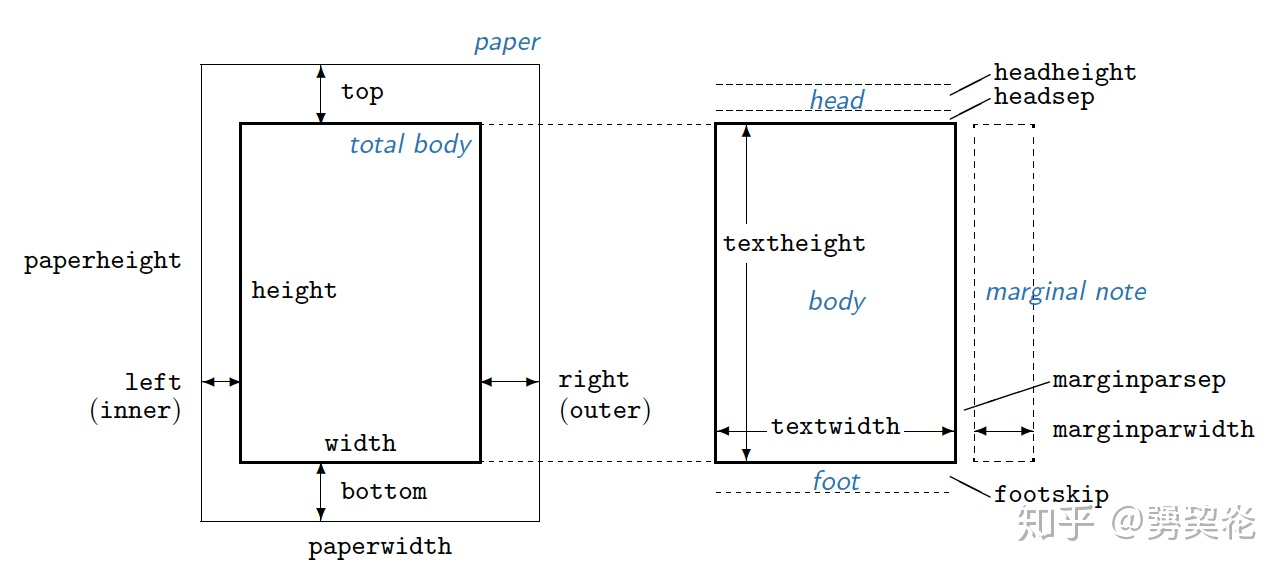
\includegraphics[width=0.8\textwidth]{fig/geometry.jpg}
    \caption{展示图}
    \label{fig:geometry}
\end{figure}

\section{本章小结}

接着编
\chapter{圆圆}

\section{本章小节}
\label{sec:deep-summary}

猫猫的由来

猫猫的待遇

猫猫的离开
\chapter{贡献二}

加油写啊

\section{本章小节}

冲啊
\chapter{妈妈}
\label{ch:contrastive}

第三个创新点写完了吗

\section{本章小节}
\label{sec:contrastive-summary}

初为人母的感受

母乳的过程

平和的启程
\chapter{总结与展望}

\section{本文总结}

众生平等

\section{未来工作}

更多细节等你发现

% ======================================================================= %
\newpage
\phantomsection
\addcontentsline{toc}{chapter}{参考文献}
\bibliographystyle{gbt7714-numerical}
\bibliography{bib/ref}
% \begin{thebibliography}{zz}

% \bibitem{2000Joux}
% Joux, Antoine. "A one round protocol for tripartite Diffie–Hellman."Algorithmic number theory. Springer Berlin Heidelberg, 2000. 385-393.

% \bibitem{2001Boneh}
% Boneh, Dan, and Matt Franklin. "Identity-based encryption from the Weil pairing." Advances in Cryptology—CRYPTO 2001. Springer Berlin Heidelberg, 2001.

% \bibitem{1984S}
% Identity-Based Cryptosystems and Signature Schemes

% \bibitem{2003J}
% J.C.Cha,J.H.Cheon.An identity-based signature from gap Diffie-Hellman groups.In Y Desmedt,editor,Public Key Cryptography-PKC 2003,LNCS 2567,Berlin:Springer-Verlag,2003:18-30

% \end{thebibliography}



\phantomsection
\addcontentsline{toc}{chapter}{致谢}
\chapter*{致\qquad 谢}

{\fangsong
谢导师不扣之恩。
}

\phantomsection
\addcontentsline{toc}{chapter}{硕士期间发表的学术论文以及学术成果}
\chapter*{\large 硕士期间发表的学术论文以及学术成果}

\renewcommand{\labelenumi}{[\arabic{enumi}]}

\subsection*{学术论文和出版物}

\begin{enumerate}	
	\item \anos{\textbf{Me}, Tutor}{(第一作者)}: Title[C] // Conference. 2021. (CCF B, Accepted)

\end{enumerate} 

\subsection*{参与基金项目}

\begin{enumerate}
	\item 国家自然科学面上项目 “学会做人” (No. 666)
\end{enumerate}


\end{document}

